%LaTeX template : http://systbio.org/files/SB_LaTeX_Template_txt_extension.txt
%Author instructions: http://www.oxfordjournals.org/our_journals/sysbio/for_authors/ms_preparation.html

\documentclass[12pt,letterpaper]{article}
\usepackage{natbib}

%Packages
\usepackage{pdflscape}
\usepackage{fixltx2e}
\usepackage{textcomp}
\usepackage{fullpage}
\usepackage{float}
\usepackage{latexsym}
\usepackage{url}
\usepackage{epsfig}
\usepackage{graphicx}
\usepackage{amssymb}
\usepackage{amsmath}
\usepackage{bm}
\usepackage{array}
\usepackage[version=3]{mhchem}
\usepackage{ifthen}
\usepackage{caption}
\usepackage{hyperref}
\usepackage{amsthm}
\usepackage{amstext}
\usepackage{enumerate}
\usepackage[osf]{mathpazo}
\usepackage{dcolumn}
\usepackage{lineno}
\usepackage{dcolumn}
\newcolumntype{d}[1]{D{.}{.}{#1}}

\pagenumbering{arabic}


%Pagination style and stuff
\linespread{2}
\raggedright
\setlength{\parindent}{0.5in}
\setcounter{secnumdepth}{0} 
\renewcommand{\section}[1]{%
\bigskip
\begin{center}
\begin{Large}
\normalfont\scshape #1
\medskip
\end{Large}
\end{center}}
\renewcommand{\subsection}[1]{%
\bigskip
\begin{center}
\begin{large}
\normalfont\itshape #1
\end{large}
\end{center}}
\renewcommand{\subsubsection}[1]{%
\vspace{2ex}
\noindent
\textit{#1.}---}
\renewcommand{\tableofcontents}{}

\begin{document}

%Running head
\begin{flushright}
Version dated: \today
\end{flushright}
\bigskip
\noindent RH: Cretaceous-Palaeogene extinction does not affect mammalian disparity.

\bigskip
\medskip
\begin{center}

\noindent{\Large \bf Cretaceous-Palaeogene extinction does not affect mammalian disparity.} 
% NC: still think this might need some work

\bigskip

\noindent {\normalsize \sc Thomas Guillerme$^1$$^,$$^2$$^*$, and Natalie Cooper$^1$$^,$$^2$$^,$$^3$}\\
\noindent {\small \it 
$^1$School of Natural Sciences, Trinity College Dublin, Dublin 2, Ireland.\\
$^2$Trinity Centre for Biodiversity Research, Trinity College Dublin, Dublin 2, Ireland.\\
$^3$Department of Life Sciences, Natural History Museum, Cromwell Road, London, SW7 5BD, UK.}\\
\end{center}
\medskip
\noindent{*\bf Corresponding author.} \textit{Zoology Building, Trinity College Dublin, Dublin 2, Ireland; E-mail: guillert@tcd.ie; Fax: +353 1 6778094; Tel: +353 1 896 2571.}\\
\vspace{1in}

%Line numbering
\modulolinenumbers[1]
\linenumbers

\renewcommand\thefigure{S\arabic{figure}}
\renewcommand\thetable{S\arabic{table}}

\section{Supplementary results}

\subsection{Phylogenies}
This section contains the trimmed phylogenies used in the analysis (see methods section in the main text for details).
\begin{figure}[!htbp]
\centering
    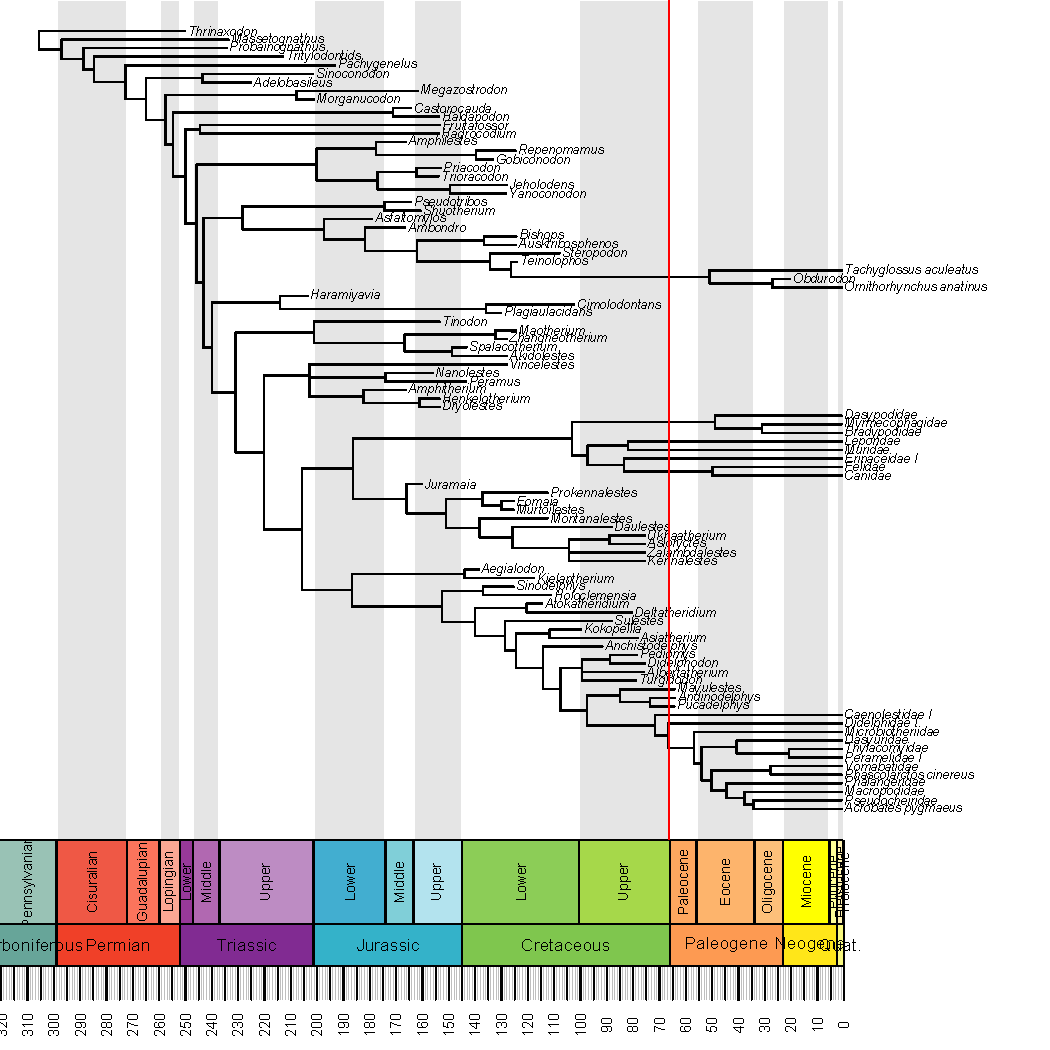
\includegraphics[keepaspectratio=true]{Figures/Slater_tree.pdf}
\caption{Mammaliaformes phylogeny from \cite{Slater2012MEE}. The phylogeny only contains taxa with overlapping cladistic data. The vertical red line represents the K-Pg boundary.}
\end{figure}

\begin{figure}[!htbp]
\centering
    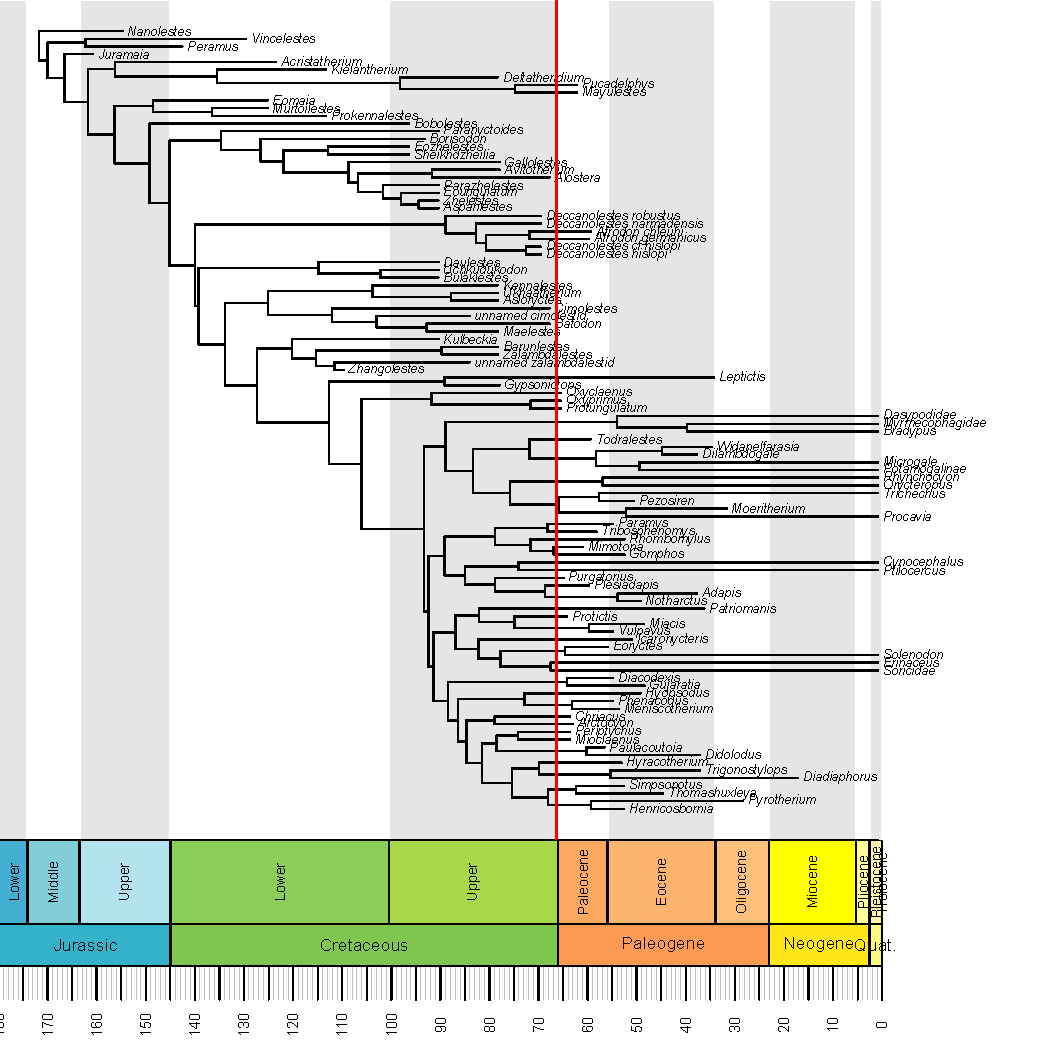
\includegraphics[keepaspectratio=true]{Figures/Beck_tree.pdf}
\caption{Eutherian phylogeny from \cite{beckancient2014}. The phylogeny only contains taxa with overlapping cladistic data. The vertical red line represents the K-Pg boundary.}
\end{figure}

\subsection{Rarefied Eutherian disparity}
This section contains the fully rarefied data set from \cite{beckancient2014} (see methods section in the main text for details).

\begin{figure}[!htbp]
\centering
    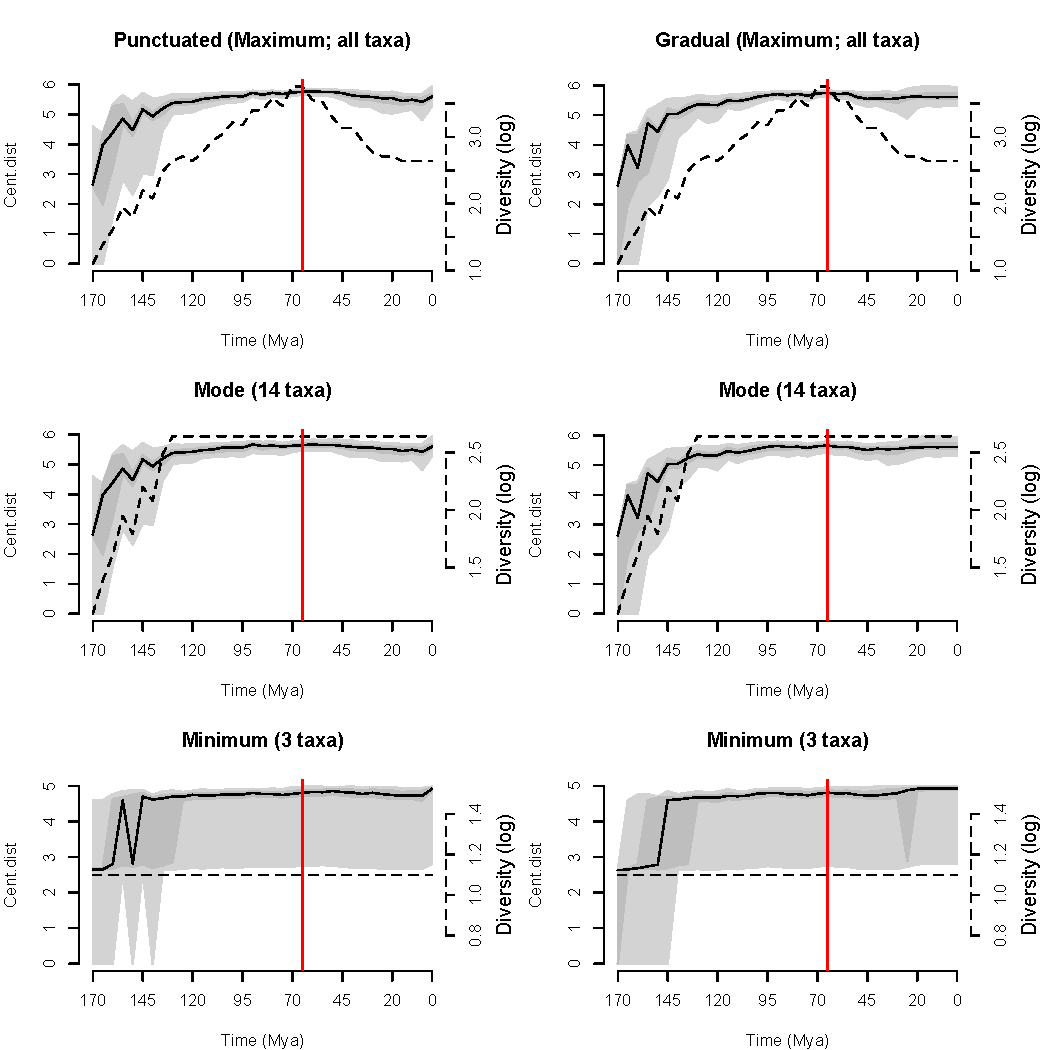
\includegraphics[keepaspectratio=true]{Figures/Rarefaction(beck).pdf}
\caption{Variations of disparity through time among Eutherian with a punctuated or gradual evolution model for different number of taxa (rarefaction). The x axis represents the time in Million of years ago (Mya). The y axis represents the disparity measured as the median distance from centroid per sub-sample. The solid black lines is the mean disparity; the confidence intervals (CI) are represent by the grey polygons (50\% CI in dark grey and 95\% CI in light grey). The dashed line represent the species richness in each sub-sample (values are reported on the right hand side of each graphs). The red vertical line represents the K-Pg boundary (66 Mya).}
\end{figure}

\subsection{Other disparity measurements}
This section contains the results of the analysis of the Mammaliaformes and Eutherian data set with all the disparity measurements and methods for sampling disparity through time.
The different disparity measurements are the median distance from centroid (see methods section in the main text for details) as well as the median sum and products of ranges and variances from \cite{Wills1994}.
The different methods for sampling disparity through time are:
\begin{enumerate}
\item \textbf{Intervals (tips only)}. We selected every tips present at every stages from the early Middle Jurassic (Bajocian, starting at 170.3 Mya) to the present. We collapsed together every stage containing less than 3 tips. Note that some tips where present in multiple stages due to their occurrence data (see methods section in the main text for details on the occurrence data).
\item \textbf{Intervals (tips and nodes)}. We selected every stage tips and nodes present at every stages from the early Middle Jurassic (Bajocian, starting at 170.3 Mya) to the present. We collapsed together every stage containing less than 3 elements (tips and/or nodes).
\item \textbf{Slices (punctuated)}. These are the results presented in the main text where time is sample equidistantly and evolution is assumed to be punctuated (randomly selecting either data from the descendant or the ancestor when slicing through a branch; see methods section in the main text for details).
\item \textbf{Slices (punctuated: acctran)}. Similar as slices (punctuated) method but data is always selected from the descendant (see methods section in the main text for details).
\item \textbf{Slices (punctuated: deltran)}. Similar as slices (punctuated) method but data is always selected from the ancestor (see methods section in the main text for details).
\item \textbf{Slices (gradual)}. SThese are the results presented in the main text where time is sample equidistantly and evolution is assumed to be gradual (data is selected from the descendant or the ancestor based on branch length; see methods section in the main text for details).
\end{enumerate}
We also rarefied both data sets for all the metrics and all the methods using only 3 taxa for the interval methods and 8 taxa for the slices methods.


\begin{landscape}
\begin{figure}[!htbp]
\centering
    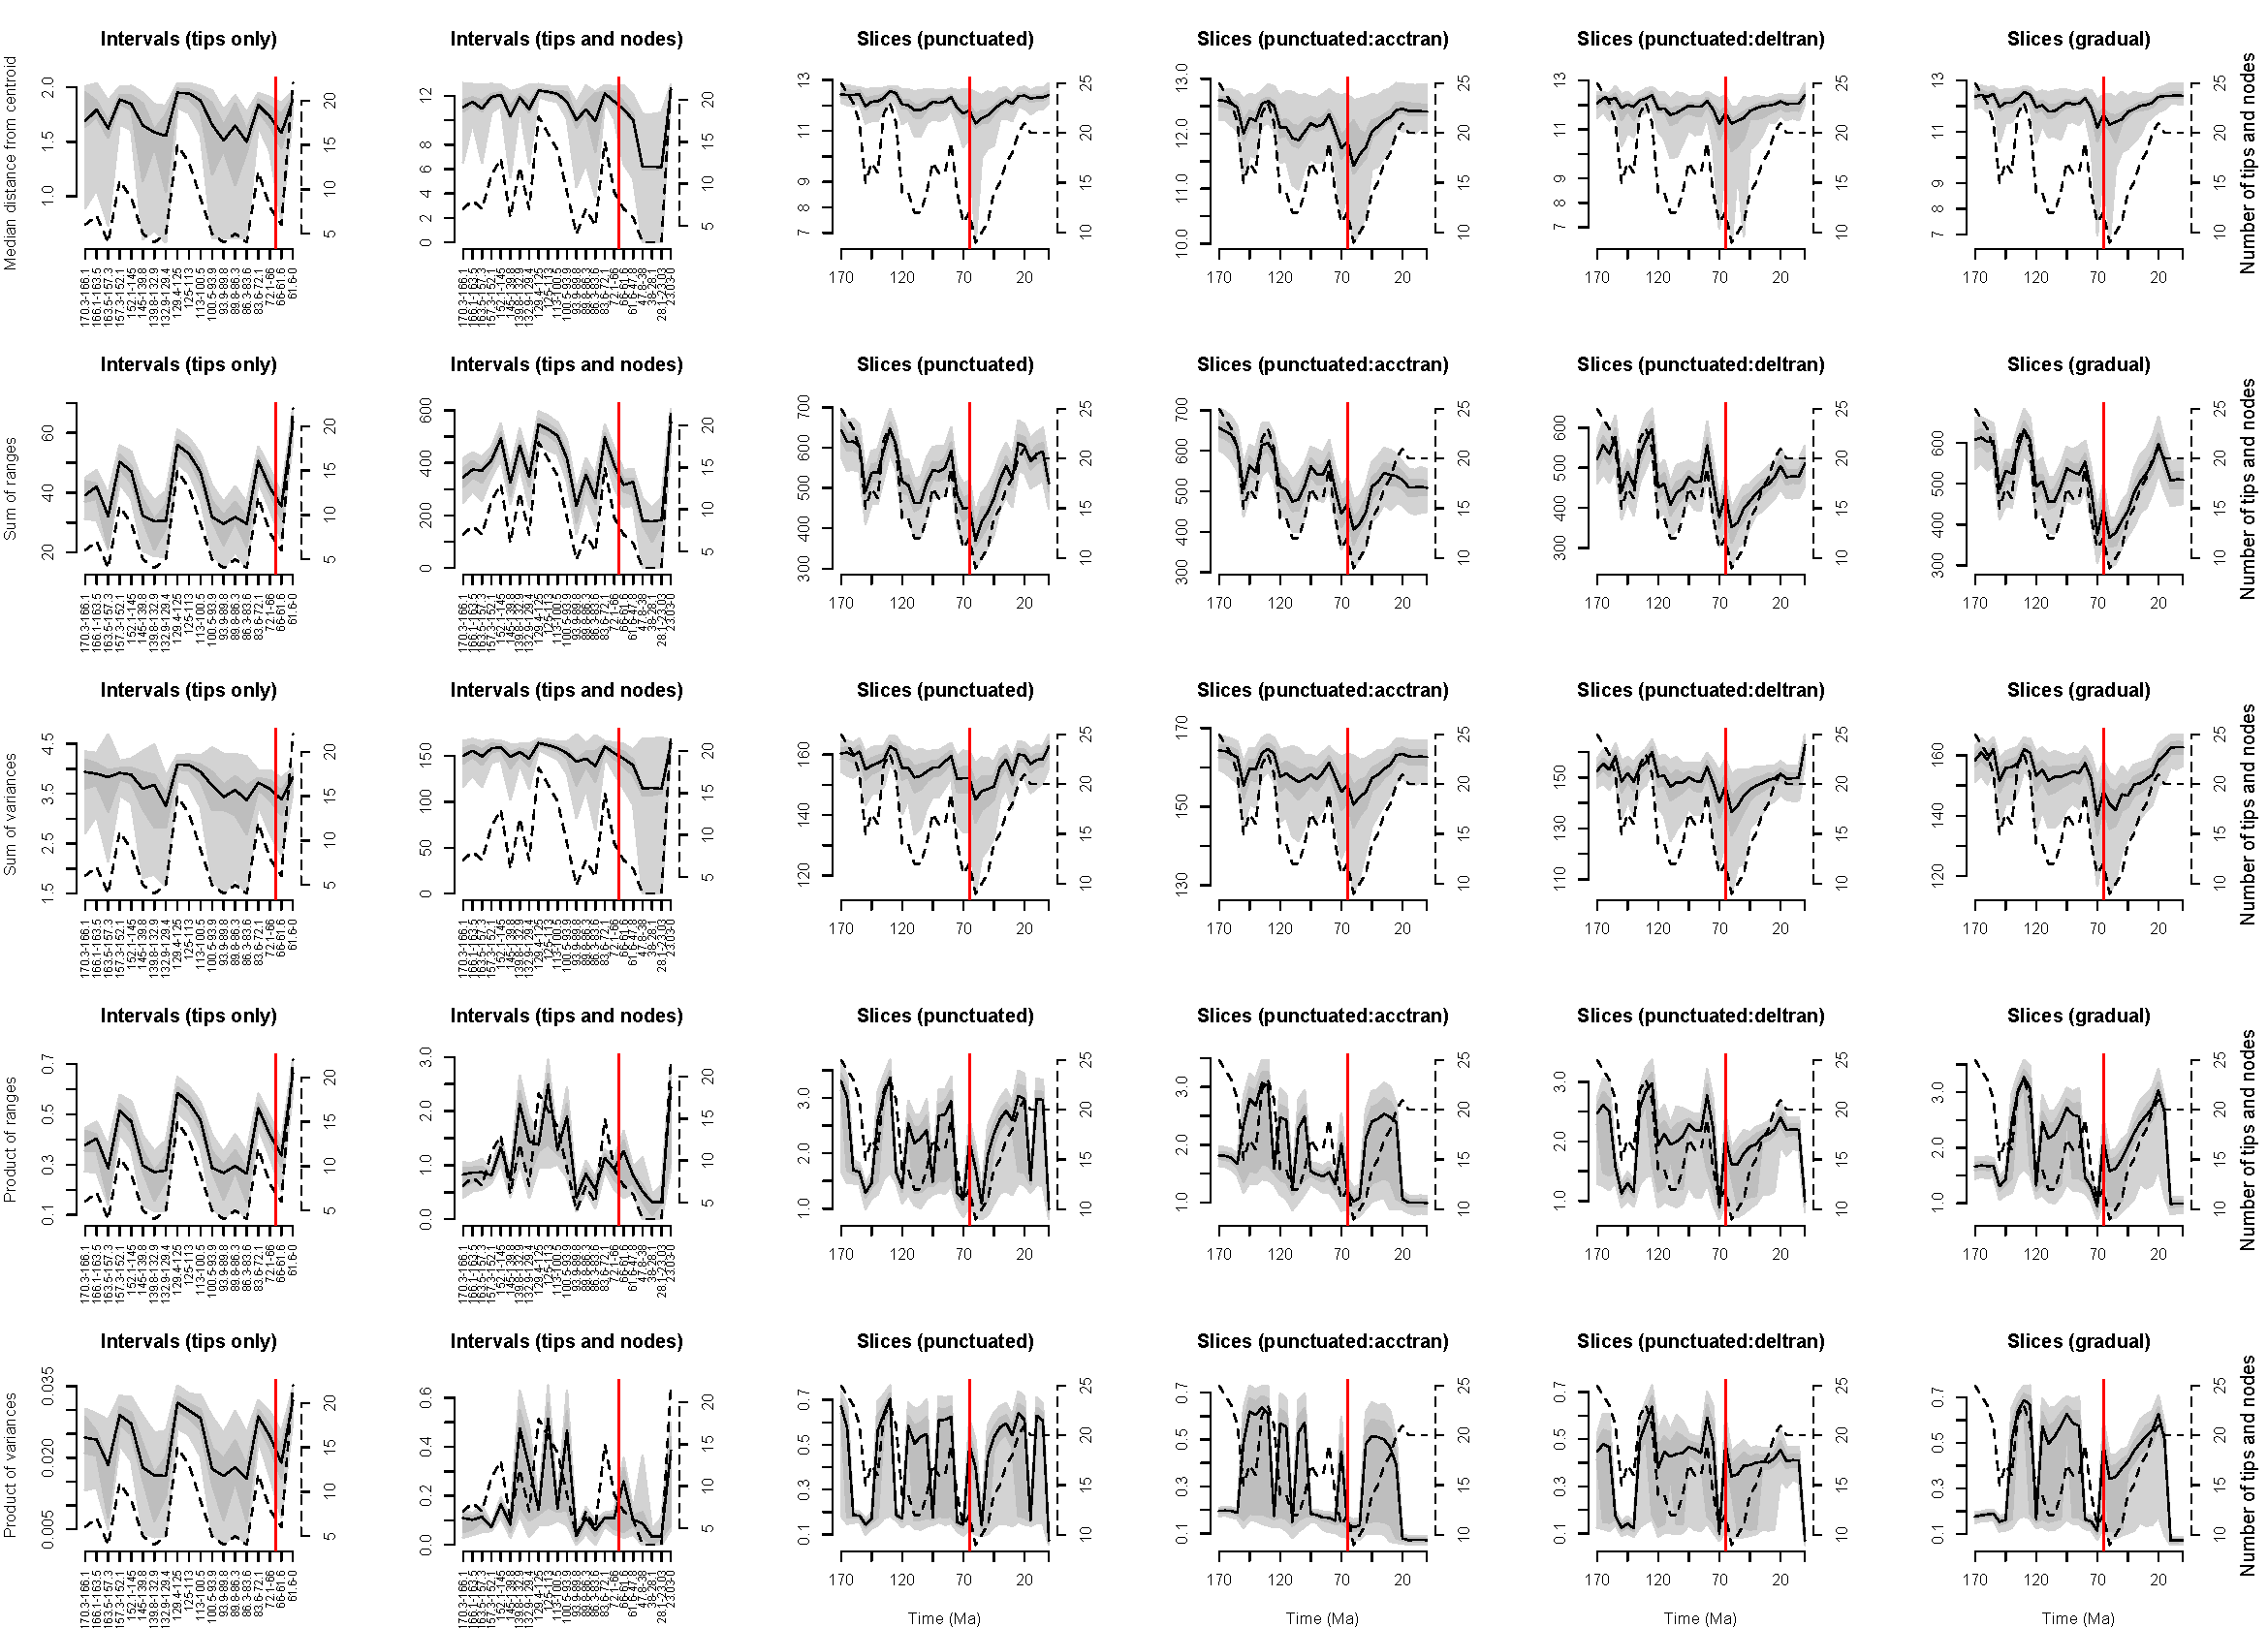
\includegraphics[width=\textwidth,height=\textheight,keepaspectratio]{Figures/Mammaliaformes(slater)_all_methods.pdf}
\caption{Variations of disparity through time among Mammaliaformes with disparity measurements and methods for sampling disparity through time. The x axis represents the time in Million of years ago (Mya). The y axis represents the disparity measured as the median distance from centroid per sub-sample. The solid black lines is the mean disparity; the confidence intervals (CI) are represent by the grey polygons (50\% CI in dark grey and 95\% CI in light grey). The dashed line represent the species richness in each sub-sample (values are reported on the right hand side of each graphs). The red vertical line represents the K-Pg boundary (66 Mya).}
\end{figure}
\end{landscape}

\begin{landscape}
\begin{figure}[!htbp]
\centering
    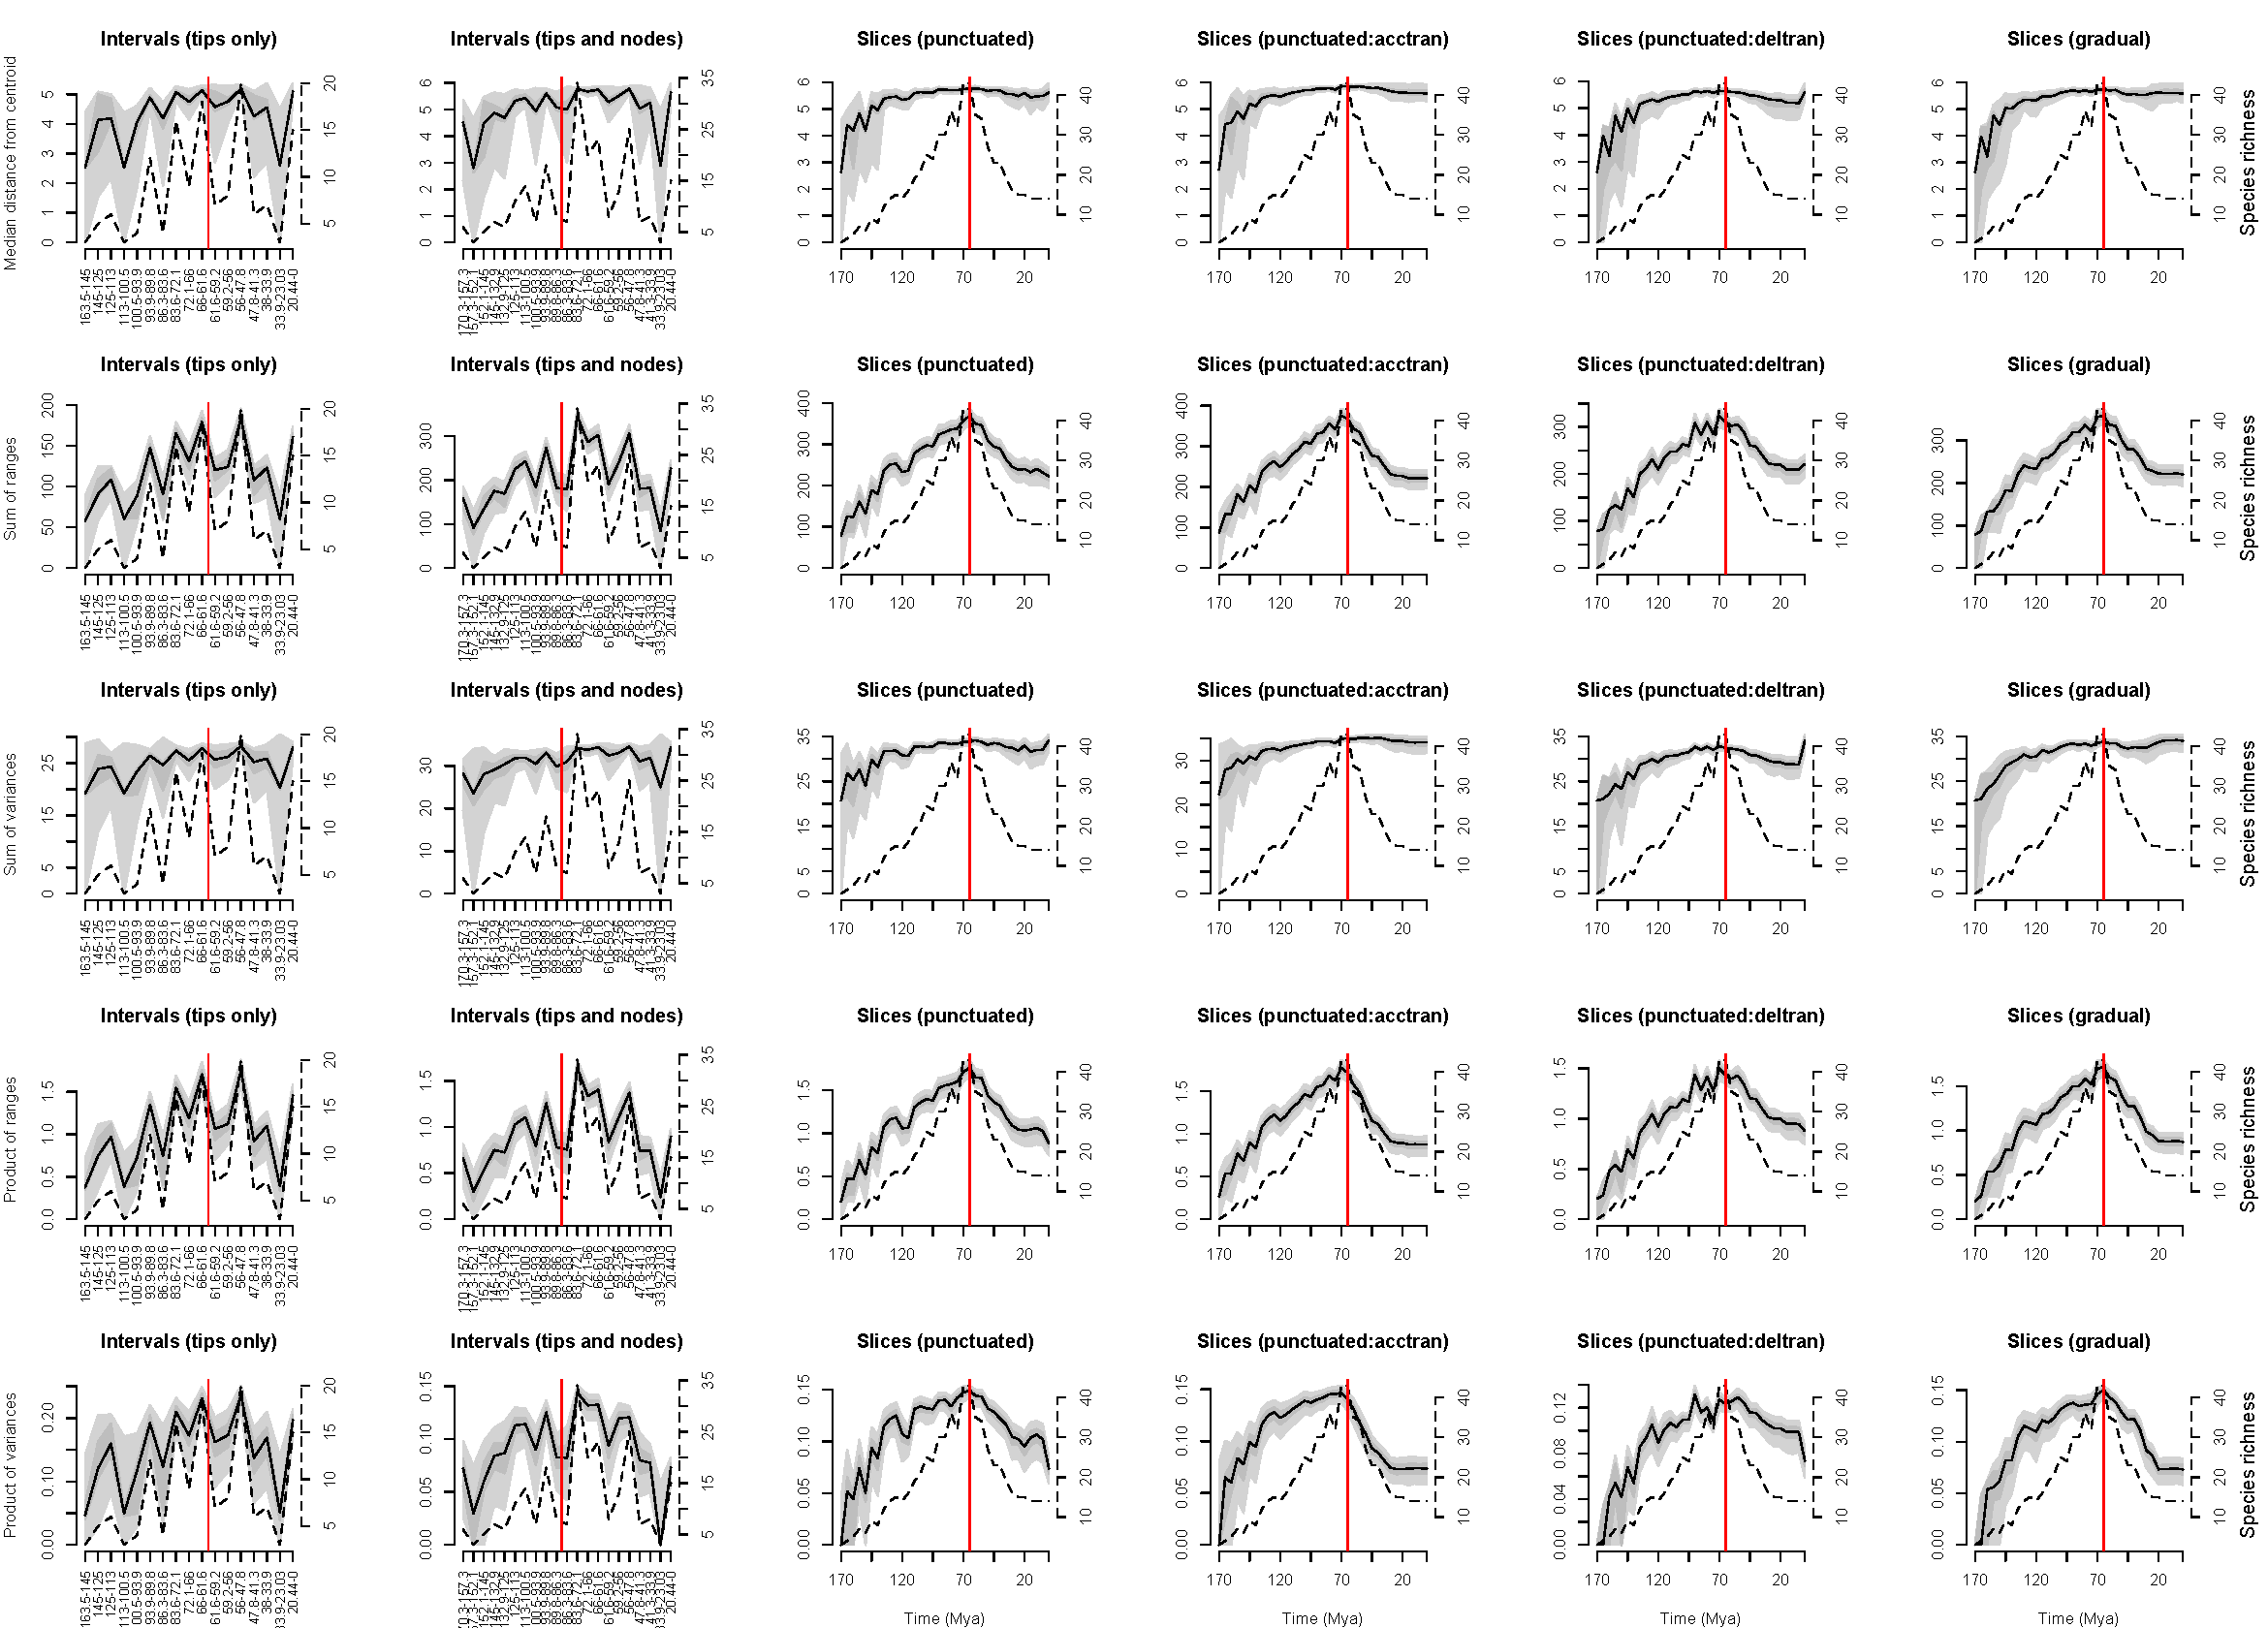
\includegraphics[width=\textwidth,height=\textheight,keepaspectratio]{Figures/Eutheria(beck)_all_methods.pdf}
\caption{Variations of disparity through time among Eutherian with disparity measurements and methods for sampling disparity through time. The x axis represents the time in Million of years ago (Mya). The y axis represents the disparity measured as the median distance from centroid per sub-sample. The solid black lines is the mean disparity; the confidence intervals (CI) are represent by the grey polygons (50\% CI in dark grey and 95\% CI in light grey). The dashed line represent the species richness in each sub-sample (values are reported on the right hand side of each graphs). The red vertical line represents the K-Pg boundary (66 Mya).}
\end{figure}
\end{landscape}

\begin{landscape}
\begin{figure}[!htbp]
\centering
    \includegraphics[width=\textwidth,height=\textheight,keepaspectratio]{Figures/Mammaliaformes(slater)_all_methods_rarefied.pdf}
\caption{Variations of disparity through time among Mammaliaformes with disparity measurements and methods for sampling disparity through time (rarefied with 3 taxa for the interval method and 8 taxa for the slice method). The x axis represents the time in Million of years ago (Mya). The y axis represents the disparity measured as the median distance from centroid per sub-sample. The solid black lines is the mean disparity; the confidence intervals (CI) are represent by the grey polygons (50\% CI in dark grey and 95\% CI in light grey). The dashed line represent the species richness in each sub-sample (values are reported on the right hand side of each graphs). The red vertical line represents the K-Pg boundary (66 Mya).}
\end{figure}
\end{landscape}

\begin{landscape}
\begin{figure}[!htbp]
\centering
    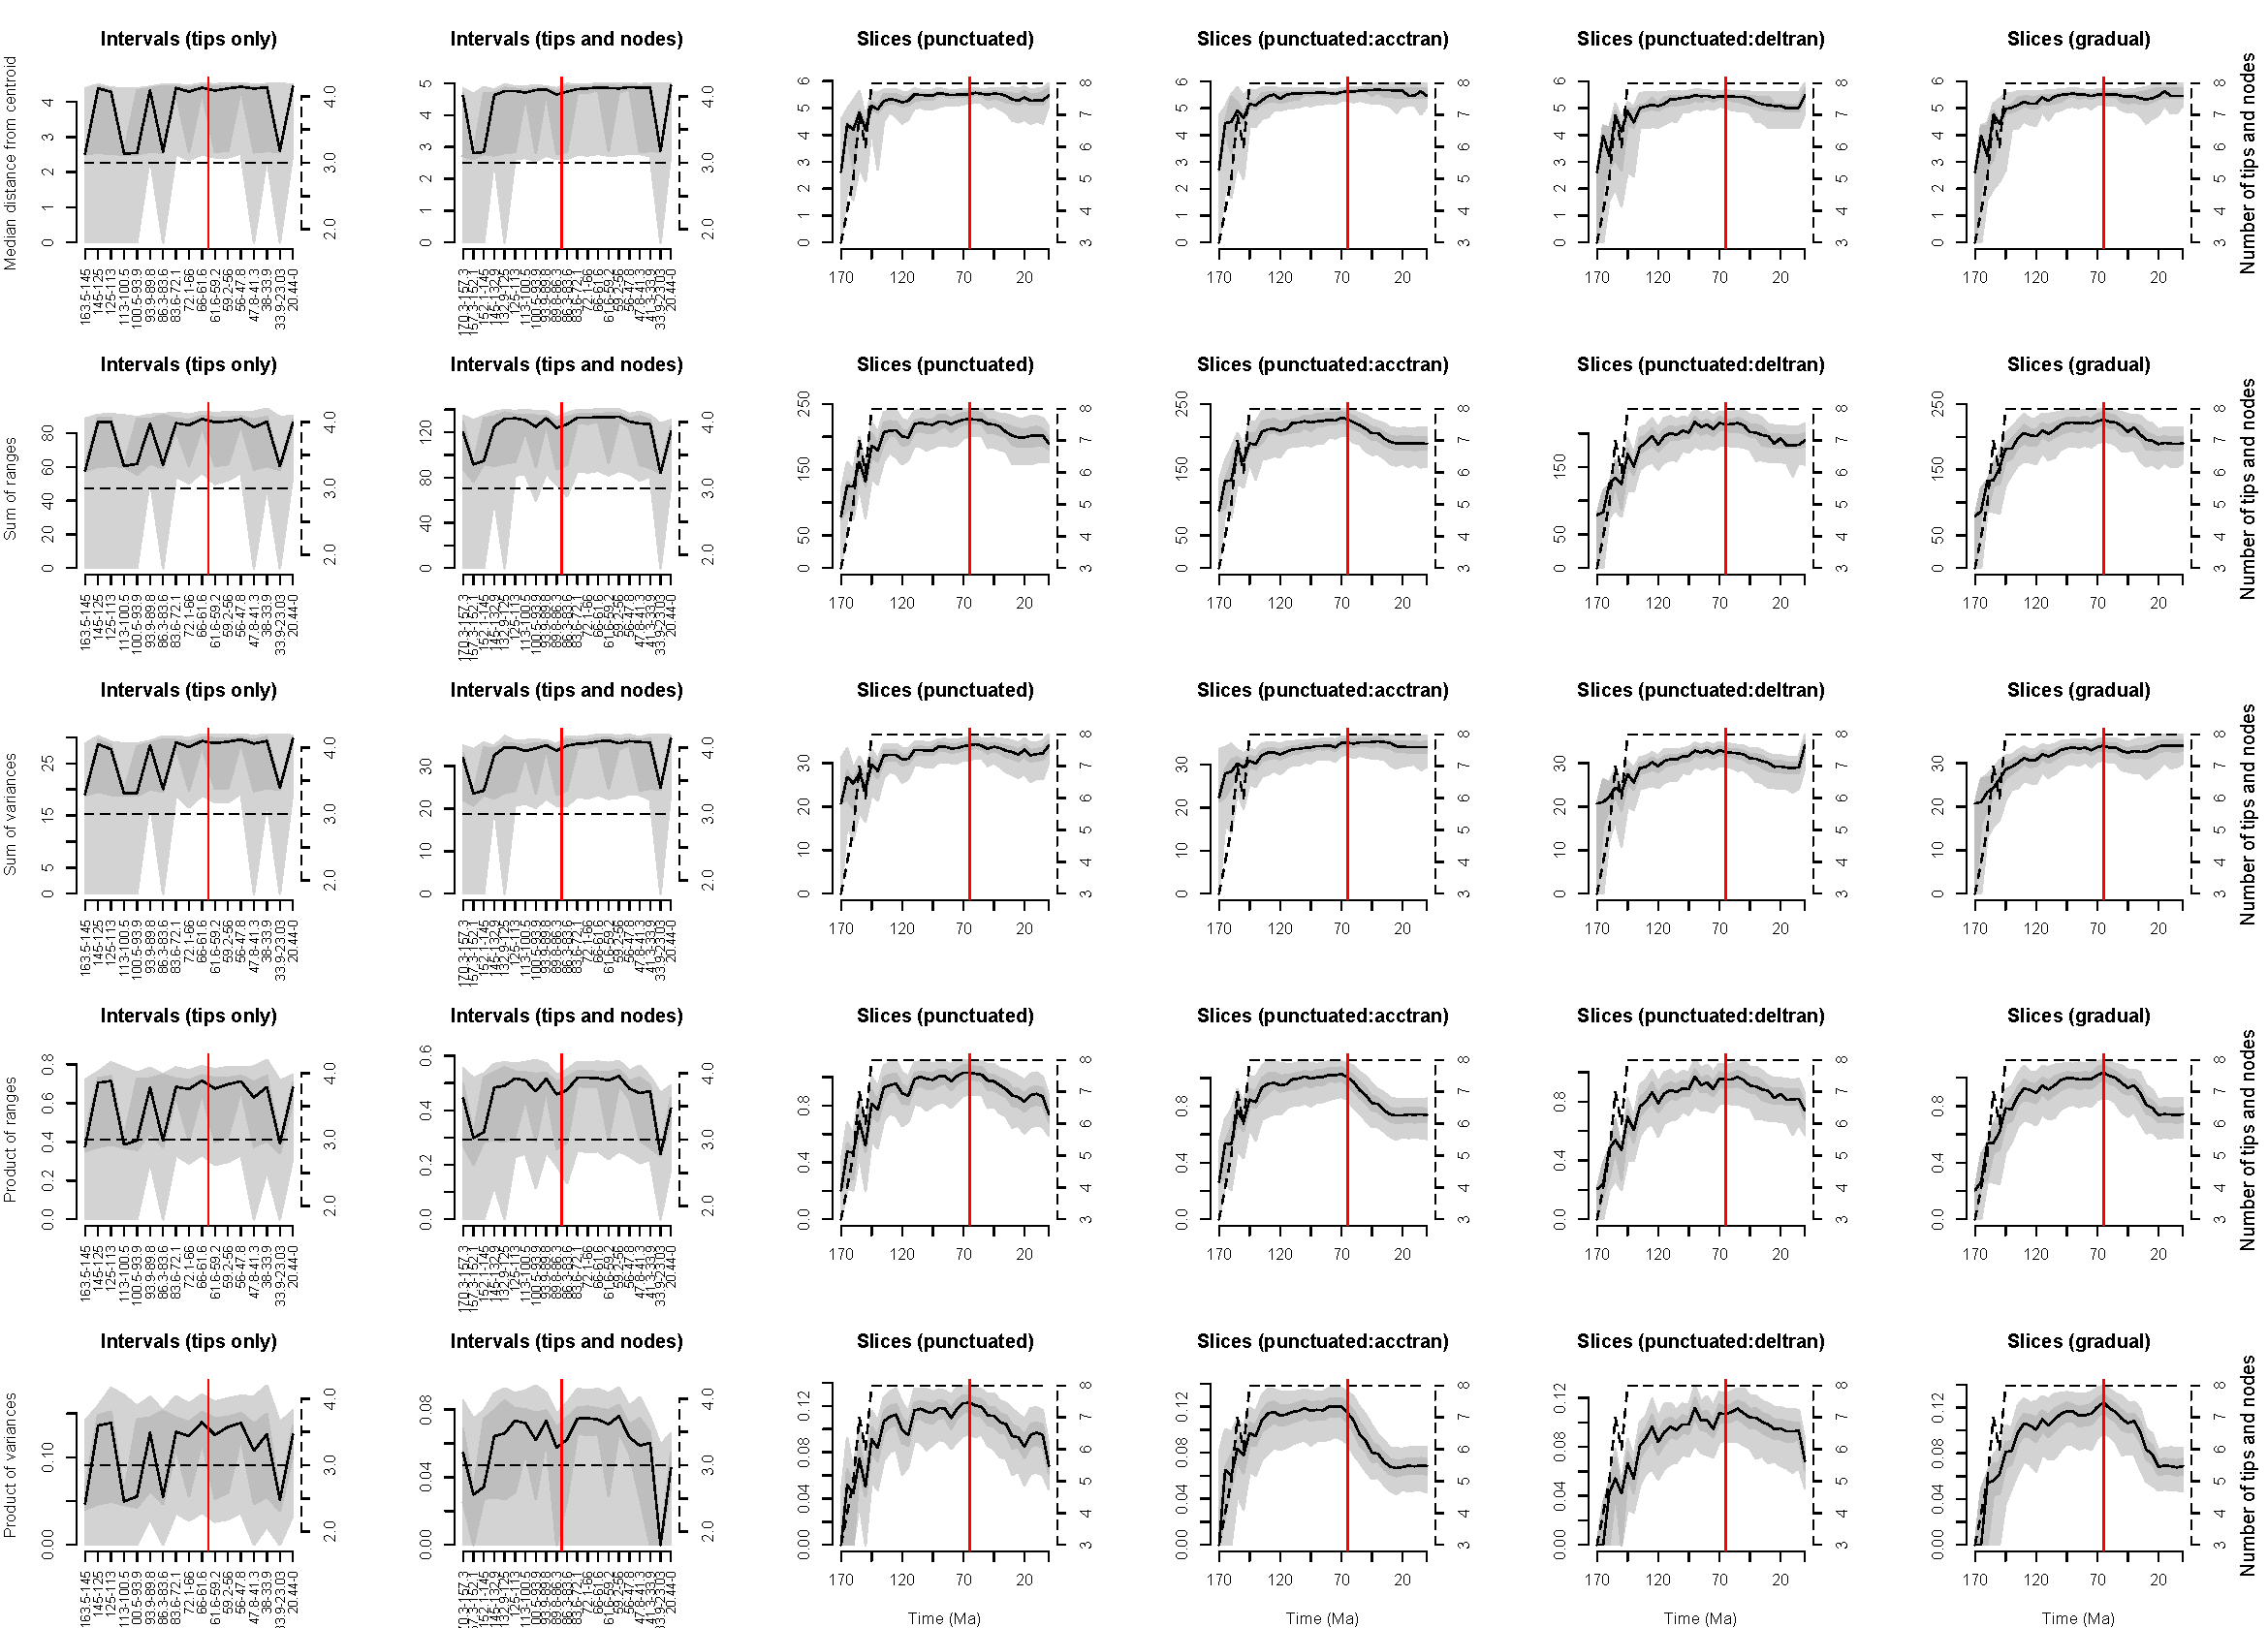
\includegraphics[width=\textwidth,height=\textheight,keepaspectratio]{Figures/Eutheria(beck)_all_methods_rarefied.pdf}
\caption{Variations of disparity through time among Eutherian with disparity measurements and methods for sampling disparity through time (rarefied with 3 taxa for the interval method and 8 taxa for the slice method). The x axis represents the time in Million of years ago (Mya). The y axis represents the disparity measured as the median distance from centroid per sub-sample. The solid black lines is the mean disparity; the confidence intervals (CI) are represent by the grey polygons (50\% CI in dark grey and 95\% CI in light grey). The dashed line represent the species richness in each sub-sample (values are reported on the right hand side of each graphs). The red vertical line represents the K-Pg boundary (66 Mya).}
\end{figure}
\end{landscape}

\subsection{Statistical test}
We applied the Permutational Analysis of Variance \citep{permanova} and the \textit{post-hoc} t-test (following \citealt{Anderson2011}) as described in the main text (see methods) on all the disparity measurements and all the methods for sampling disparity through time.
The results are available in .csv file available here (ADD THE LINK).
Note that it was not possible to perform any \textit{post-hoc} t-test for the product of variance metric.
his was because we didn't removed any axis of the ordination based on an arbitrary value (c.f. selecting only $m$ dimensions that represent up to 90\% of the variance in the distance matrix; \citealt{Brusatte12092008,toljagictriassic-jurassic2013}) and thus, the last axis hold a really small amount of variance.
Therefore, it was computationally impossible to calculate the product of variance because the resulting values were $<$ $1$$\times$$10^{-324}$ which is treated as being equal to $0$ in \texttt{R}.




\bibliographystyle{sysbio}
\bibliography{References}


\end{document}